\documentclass[11pt]{article}

\usepackage{latexsym}
\usepackage{amsmath}
\usepackage{amssymb}
\usepackage{amsthm}
\usepackage{graphicx}
\usepackage{wrapfig}
\usepackage{pseudocode}
\usepackage{url}
\usepackage{float}
\usepackage{subcaption}
\usepackage[backref, colorlinks=true, citecolor=red, urlcolor=blue, pdfauthor={Jyh-Ming Lien}]{hyperref}


\newcommand{\handout}[5]{
  \noindent
  \begin{center}
  \framebox{
    \vbox{
      \hbox to 5.78in { {\bf } \hfill #2 }
      \vspace{4mm}
      \hbox to 5.78in { {\Large \hfill #5  \hfill} }
      \vspace{2mm}
      \hbox to 5.78in { {\em #3 \hfill #4} }
    }
  }
  \end{center}
  \vspace*{4mm}
}

\newcommand{\lecture}[4]{\handout{#1}{#2}{#3}{#4}{#1}}

\newtheorem{theorem}{Theorem}
\newtheorem{corollary}[theorem]{Corollary}
\newtheorem{lemma}[theorem]{Lemma}
\newtheorem{observation}[theorem]{Observation}
\newtheorem{proposition}[theorem]{Proposition}
\newtheorem{definition}[theorem]{Definition}
\newtheorem{claim}[theorem]{Claim}
\newtheorem{fact}[theorem]{Fact}
\newtheorem{assumption}[theorem]{Assumption}

% 1-inch margins, from fullpage.sty by H.Partl, Version 2, Dec. 15, 1988.
\topmargin 0pt
\advance \topmargin by -\headheight
\advance \topmargin by -\headsep
\textheight 8.9in
\oddsidemargin 0pt
\evensidemargin \oddsidemargin
\marginparwidth 0.5in
\textwidth 6.5in

\parindent 0in
\parskip 1.5ex
%\renewcommand{\baselinestretch}{1.25}

\begin{document}

\lecture{Project 2: Hedcut}{Fall 2019}{William Austin}{CS 633 Computational Geometry}

\section{Summary of the hedcut method}

The hedcut method that is implemented in this project is closely related to the idea of stippling, which uses a combination of dots to represent an image. Originally, this style of drawing was used in newspapers because they are typically black-and-white, can be easily printed on a page, and retained the important details of the image throughout this process. However, these works are also produced manually by a skilled artist and take several hours to complete. Therefore, this project explores how this style of art can be generated in an automated way, based off of an input image.

The provided functionality uses the concepts described in the paper ``Weighted Voronoi Stippling'', which is based on the concept of centroidal Voronoi diagrams. In order for a Voronoi diagram to be centroidal, the generating points must also be the centroid, which can be interpreted as the center of mass. For images, we can calculate the intensity at each pixel: ((R + G + B) / 3), and interpret it as a density function. Then, for each Voronoi cell, we can compute the centroid, based on the ``weight'' and location of each pixel in the cell.

The implementation is an iterative algorithm that starts off with random samples from the image. Then, we repeatedly:
\begin{enumerate}
	\item Compute the Voronoi diagram for the given point locations, and
	\item For each cell, find the centroid, and use it as the generating point for the next iteration.
\end{enumerate}

We must introduce some stopping criteria so that the algorithm eventually halts. In our case, we can specify an upper limit to the number of iterations performed or the distance the centroid moves in a step (total or average.) 

\section{Improvement of hedcuter method}

I've made several improvements to the provided functionality, listed below. In each section, I will give some examples, and intuition for the new features. A quick summary of the changes is given here, in the expanded options list for the hedcuter application:

\begin{figure}[H]
	\centering
	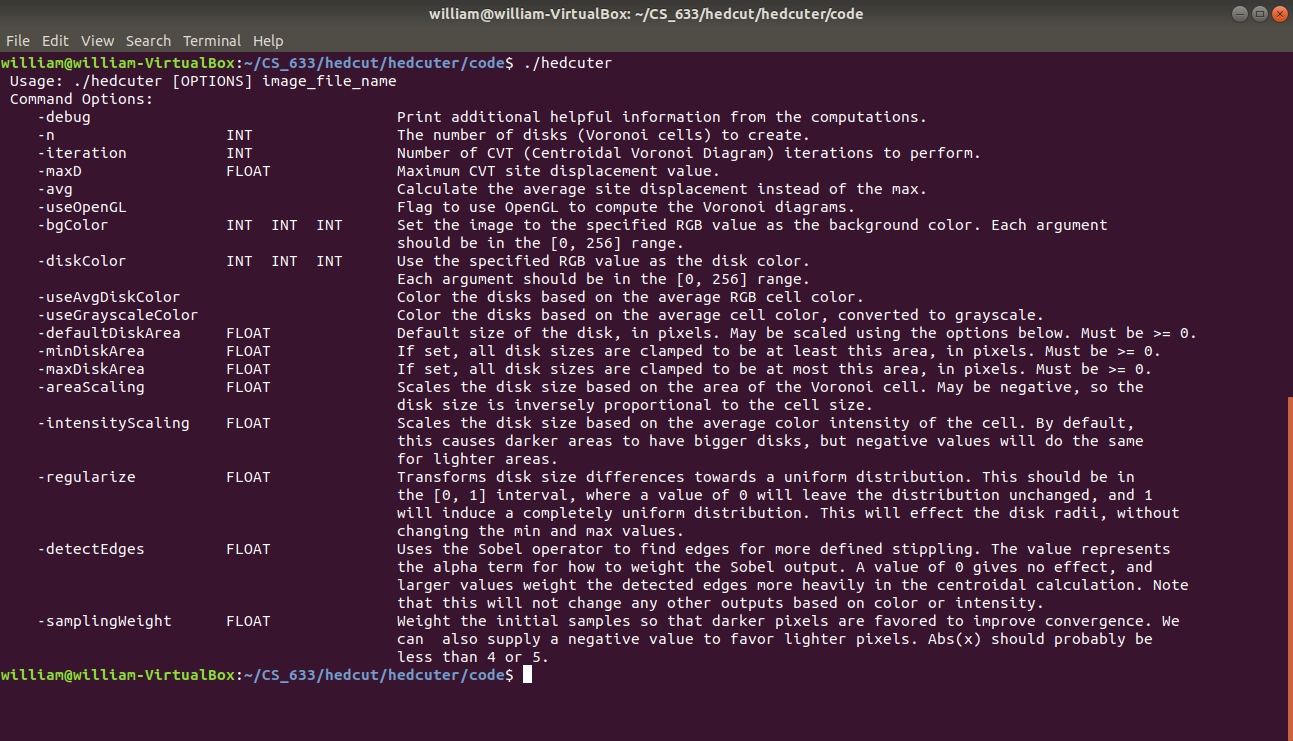
\includegraphics[scale=0.3]{HeducterCommandOptions}
	\caption{Hedcuter Application Command Options}
\end{figure}


\subsection{Creating Voronoi Diagrams using OpenGL}

The first large improvement to the application was to use OpenGL to compute the Voronoi diagrams at each step in the algorithm. The idea is to construct a scene with a cone centered on the X-Y plane at each generating point. By fixing the camera to look at the all of the cones in the direction of the Z-axis, using a 2-D projection, the resulting scene is the Voronoi diagram.

\begin{figure}[H]
	\centering
	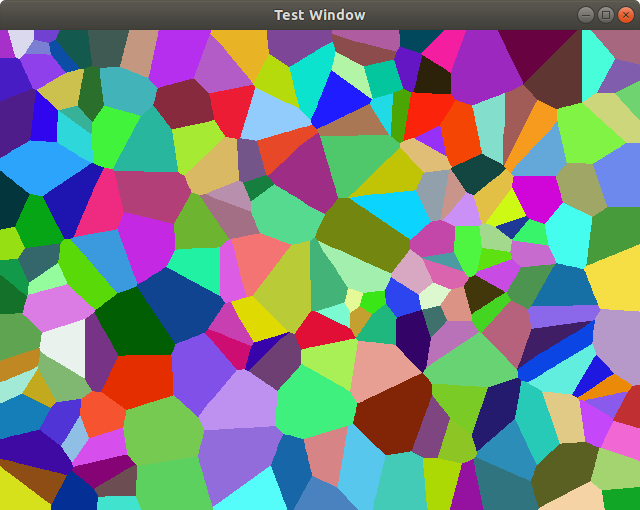
\includegraphics[scale=0.35]{VoronoiDiagram}
	\caption{Voronoi Diagram, as computed by OpenGL}
	\label{fig:voronoiDiagram}
\end{figure} 

One of the problems that arises during the implementation of this feature is trying to map the regions in the rendered diagram back to the point that generated them. We do this by converting the index of the generating point $[0 \dots n - 1]$ into the RGB color-space by transforming the index into a point in the range $[0 \dots 256^3]$, and then representing it as $256^2 \cdot R + 256 \cdot G + B$. This tells Open GL what colors to use for the cones, and then we do the reverse transform to map the Voronoi regions of a certain color back to the correct generating point.

Some other challenges that arise include:
\begin{itemize}
	\item Model space in OpenGL is represented in X-Y coordinates, so (0, 0) is in the bottom-left of the screen, whereas OpenCV uses row-column format, with the pixel at (0, 0) in the upper-left of the screen. Therefore, when converting between the representations, we must flip the image, and reverse the coordinate order.
	\item OpenGL initialization requires another library to control the window system, such as GLUT. Offline rendering does not seem to be especially well supported.
	\item Internally, the OpenCV library uses a BGR representation for colors instead of the more traditional RGB. Therefore, we need to take care to convert correctly and make sure that the code is accessing the correct channel for the data structure.
\end{itemize} 

Most of my code for this feature is in the \verb|vorgpu.hpp| and \verb|vorgpu.cpp| files. A few changes to other files were required to integrated the command line option and call the correct functionality. This is in the \verb|wcvt.cpp| file, in the \verb|compute_weighted_cvt()| function. The functionality is enabled by specifying the \verb|-useOpenGL| flag, with no options.

I was able to get good stippling results using the OpenGL option. The example below shows the original input on the left, and the generated hedcut with 4000 disks.

\begin{figure}[H]
	\centering
	\begin{subfigure}[b]{.48\linewidth}
	 	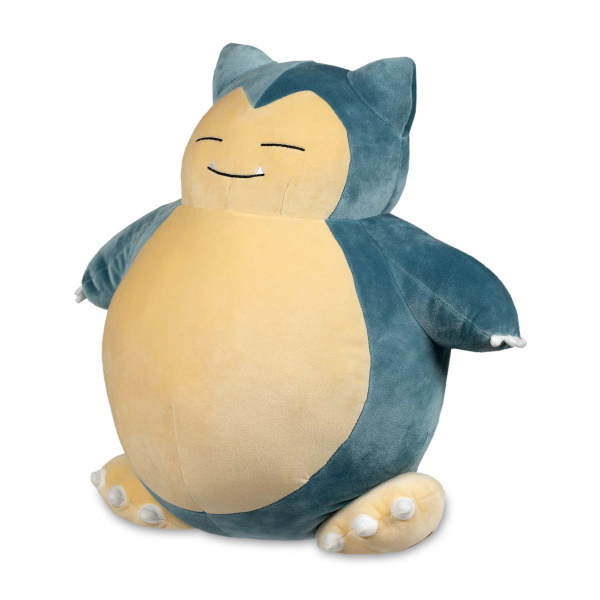
\includegraphics[width=\linewidth]{Snorlax}
	 	\caption{Original Image, Snorlax}
	 	\label{fig:snorlax}
	\end{subfigure}
	\begin{subfigure}[b]{.48\linewidth}
		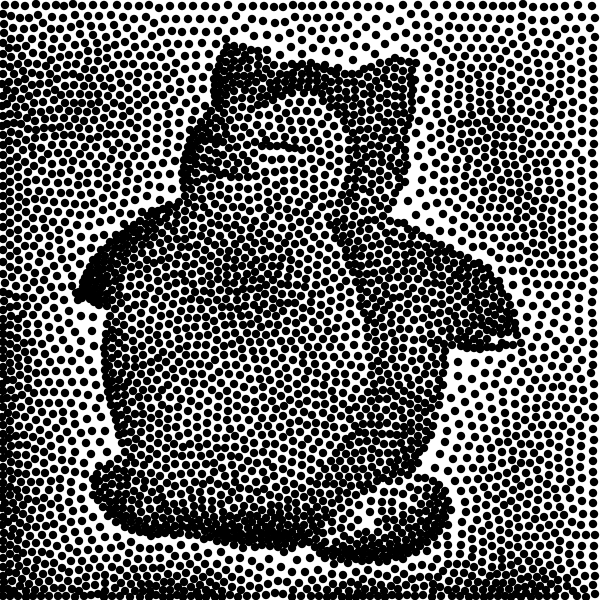
\includegraphics[width=\linewidth]{Snorlax-OpenGL-4000}
		\caption{Hedcut Image using OpenGL with 4000 Disks, Snorlax}
		\label{fig:snorlaxOpenGL}
	\end{subfigure}
	\caption{OpenGL Example with Snorlax}
	\label{fig:snorlaxExample}
\end{figure}

Despite the complete implementation and reasonable output, I did not notice a large speedup when using the OpenGL functionality instead of the built-in method. In most cases, the total time taken is comparable. For example, the output below shows that OpenGL based method was slightly slower for 750 disks.

\begin{figure}[H]
	\centering
	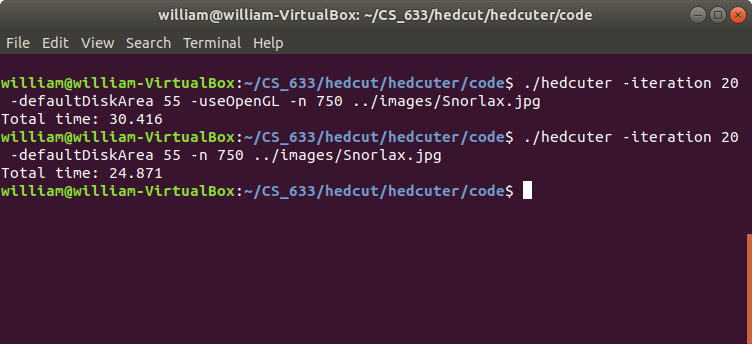
\includegraphics[scale=0.35]{OpenGL-Performance}
	\caption{Relative OpenGL Performance}
	\label{fig:OpenGLPerformance}
\end{figure} 

\subsection{Colored Disks, Grayscale Disks, and Background Color}

For the next feature to be added into the Hedcuter code, I added a few different ways to specify color in the output image. This includes:

\begin{itemize}
	\item Use the \verb|-diskColor R G B| option to specify a constant disk color. The default is black.
	\item Use the \verb|-bgColor R G B| option to specify a background color for the output. The default is no background (transparent).
	\item Use the \verb|-useGrayscaleColor| flag to create an image with disks based on the average grayscale intensity for each Voronoi cell to be represented.
	\item Use the \verb|-useAvgDiskColor| flag to create an image with disks based on the average color for each Voronoi cell to be represented.
\end{itemize} 

Some sample results are shown below.

\begin{figure}[H]
	\centering
	\begin{subfigure}[b]{.48\linewidth}
		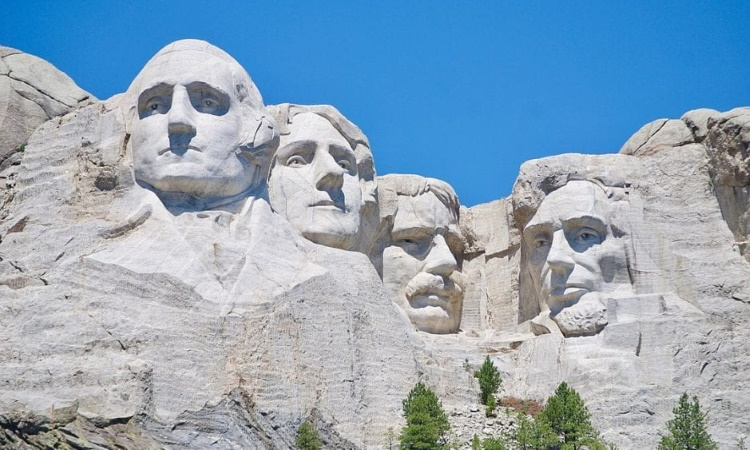
\includegraphics[width=\linewidth]{Mount-Rushmore}
		\caption{Original Image, Mount Rushmore}
		\label{fig:mountRushmore}
	\end{subfigure}
	\begin{subfigure}[b]{.48\linewidth}
		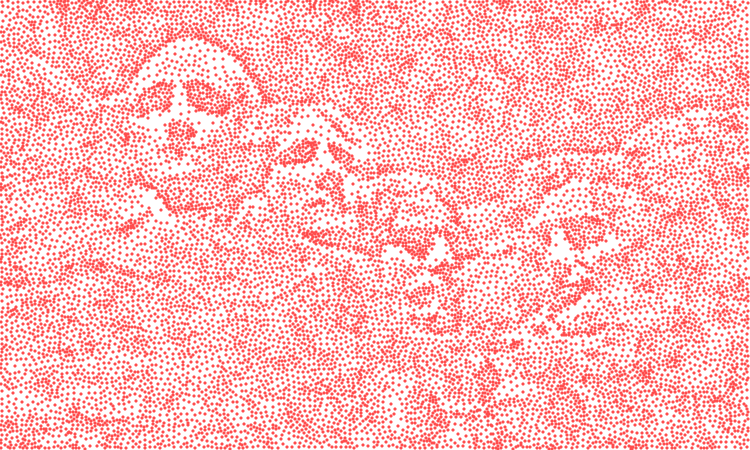
\includegraphics[width=\linewidth]{Mount-Rushmore-Red-15000}
		\caption{Red Hedcut Image with 15000 Disks}
		\label{fig:mountRusmoreRed}
	\end{subfigure}
	\begin{subfigure}[b]{.48\linewidth}
		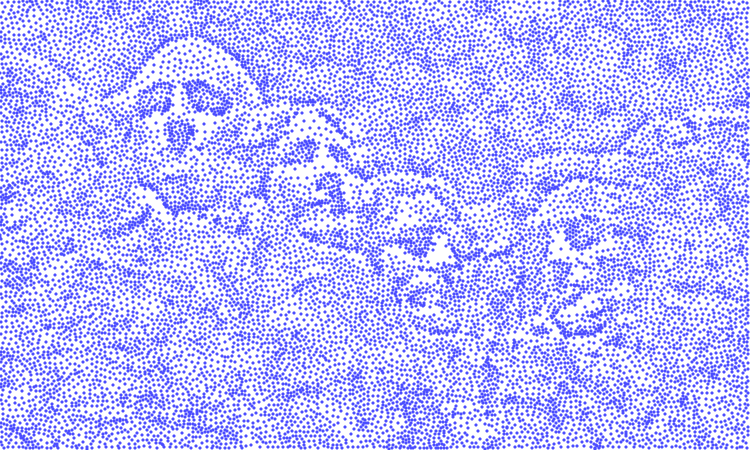
\includegraphics[width=\linewidth]{Mount-Rushmore-Blue-15000}
		\caption{Blue Hedcut Image with 15000 Disks}
		\label{fig:mountRusmoreBlue}
	\end{subfigure}
	\begin{subfigure}[b]{.48\linewidth}
		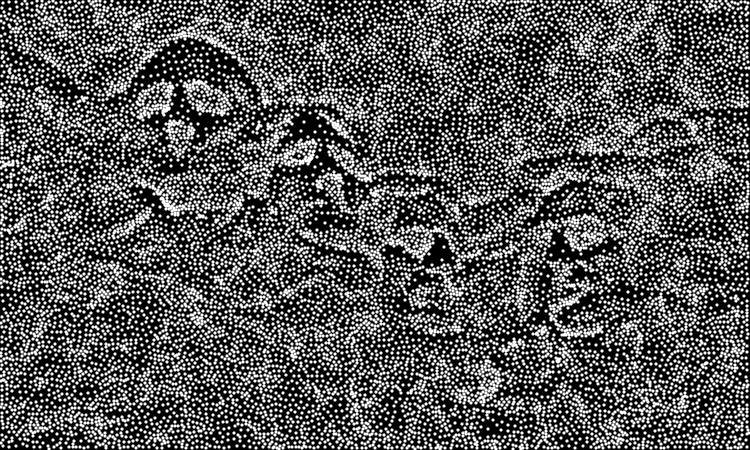
\includegraphics[width=\linewidth]{Mount-Rushmore-Inverted-15000}
		\caption{Inverted Hedcut Image with 15000 Disks}
		\label{fig:mountRusmoreInverted}
	\end{subfigure}
	\caption{Color Example with Mount Rushmore}
	\label{fig:mountRushmoreEx}
\end{figure}

A more dynamic coloring approach can be seen by using the grayscale color and average color options. This is accomplished by simply averaging all of the cell colors together to choose an approximation of the input color when we create the disks for the hedcut.

\begin{figure}[H]
	\centering
	\begin{subfigure}[b]{.52\linewidth}
		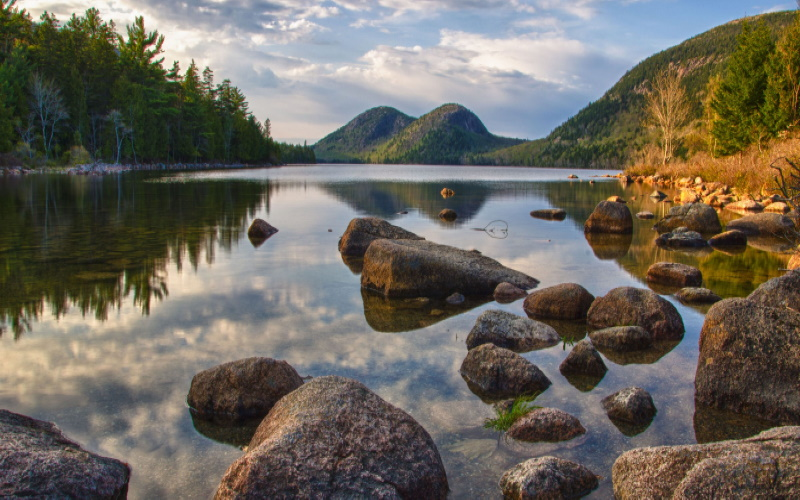
\includegraphics[width=\linewidth]{Jordan-Pond}
		\caption{Original Image, Jordan Pond}
		\label{fig:jordanPond}
	\end{subfigure}
	\begin{subfigure}[b]{.48\linewidth}
		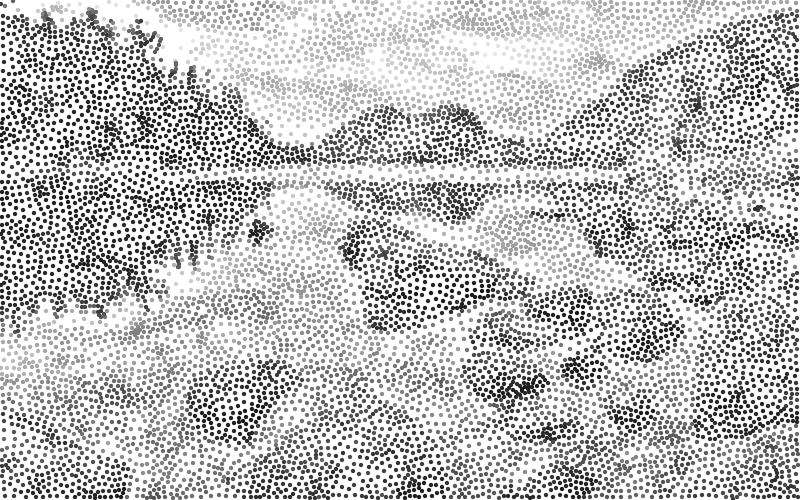
\includegraphics[width=\linewidth]{Jordan-Pond-Grayscale-10000}
		\caption{Jordan Pond, Grayscale, 10000 Disks}
		\label{fig:jordanPondGray}
	\end{subfigure}
	\begin{subfigure}[b]{.48\linewidth}
		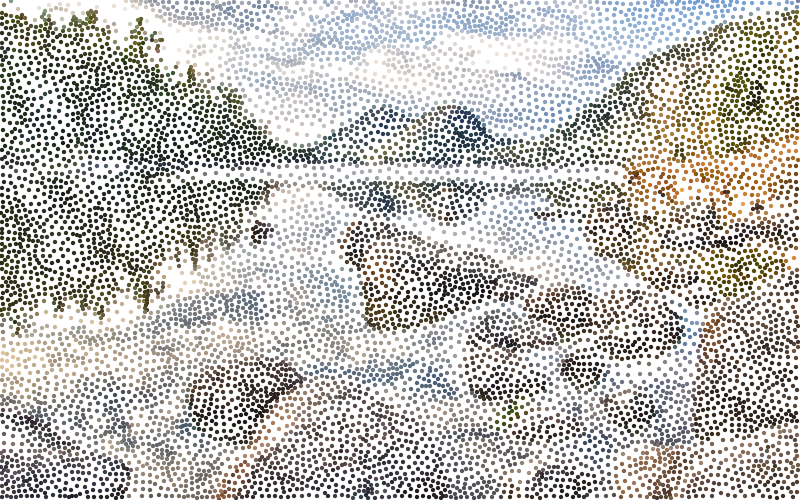
\includegraphics[width=\linewidth]{Jordan-Pond-Color-10000}
		\caption{Jordan Pond, Colored, 10000 Disks}
		\label{fig:jordanPondColor}
	\end{subfigure}
	\caption{Colore Example with Jordan Pond}
	\label{fig:jordanPondExample}
\end{figure}


\subsection{Disk Sizing based on Cell Area and Intensity, with Regularization}

I have also implemented dynamic disk sizing to produced different visual effects in the final hedcut image. The first way of doing this is to scale the size of each disk by the size of the containing Voronoi cell. This is done by specifying \verb|-areaScaling scaleFactor|. In the example with Roger Federer, you can see that the disks on the handle of the racket and his grip are much larger than the rest of the disks in the second example, but much smaller in second example because we specified a negative value to invert the relationship.

\begin{figure}[H]
	\centering
	\begin{subfigure}[b]{.52\linewidth}
		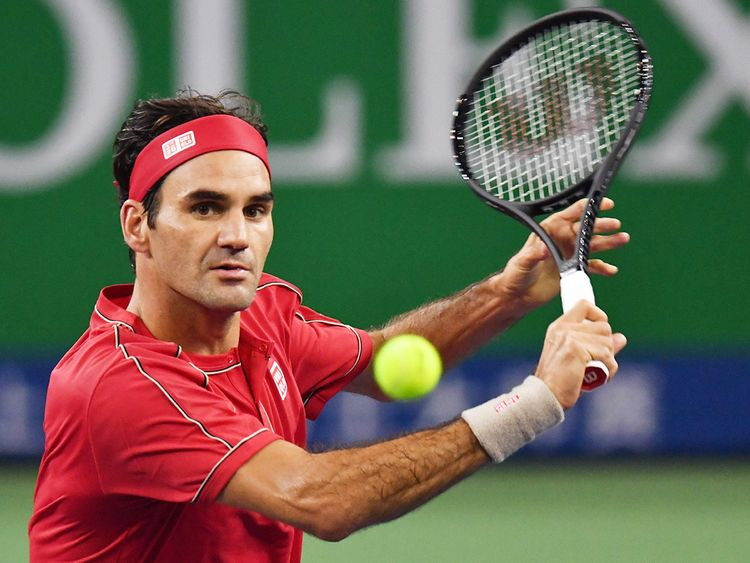
\includegraphics[width=\linewidth]{Roger-Federer}
		\caption{Original Image, Roger Federer}
		\label{fig:rf}
	\end{subfigure}
	\begin{subfigure}[b]{.48\linewidth}
		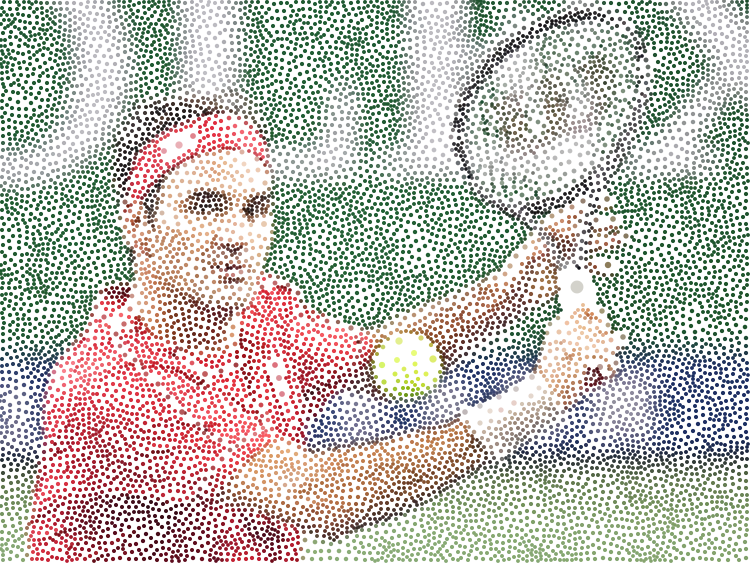
\includegraphics[width=\linewidth]{Roger-Federer-AreaScale-12000}
		\caption{Roger Federer, Area scaled, 12000 Disks}
		\label{fig:rf2}
	\end{subfigure}
	\begin{subfigure}[b]{.48\linewidth}
		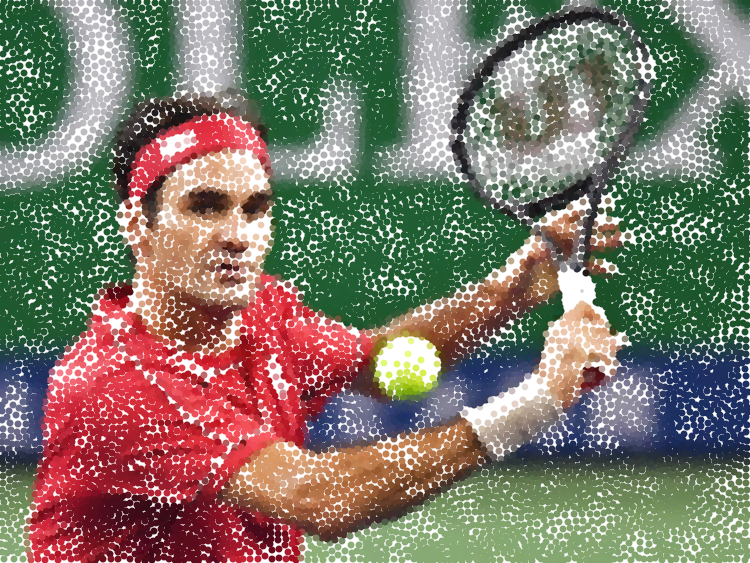
\includegraphics[width=\linewidth]{Roger-Federer-ReverseAreaScaling-12000}
		\caption{Roger Federer, Reverse area scaled, 12000 Disks}
		\label{fig:rf3}
	\end{subfigure}
	\caption{Area Scaling Example with Roger Federer}
	\label{fig:rf4}
\end{figure}

We can perform the same scaling operation, but use the average intensity of the cell as the input, instead of the cell area. This is shown below when we specify the \verb|-areaScaling scaleFactor| option. As expected, in the first image, the darker areas produce larger disks, and the lighter areas produce smaller disks. The relationship is reversed for the second example when we pass a negative argument.

\begin{figure}[H]
	\centering
	\begin{subfigure}[b]{.52\linewidth}
		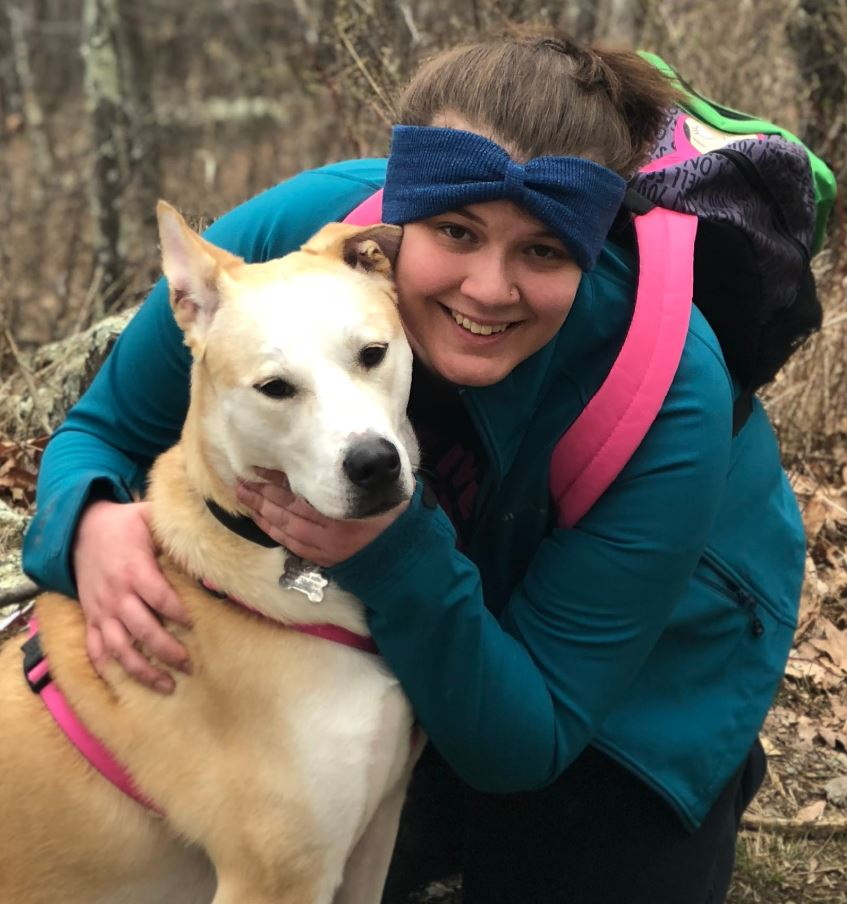
\includegraphics[width=\linewidth]{Emilee-And-Lola}
		\caption{Original Image, Girl and Dog}
		\label{fig:gff}
	\end{subfigure}
	\begin{subfigure}[b]{.48\linewidth}
		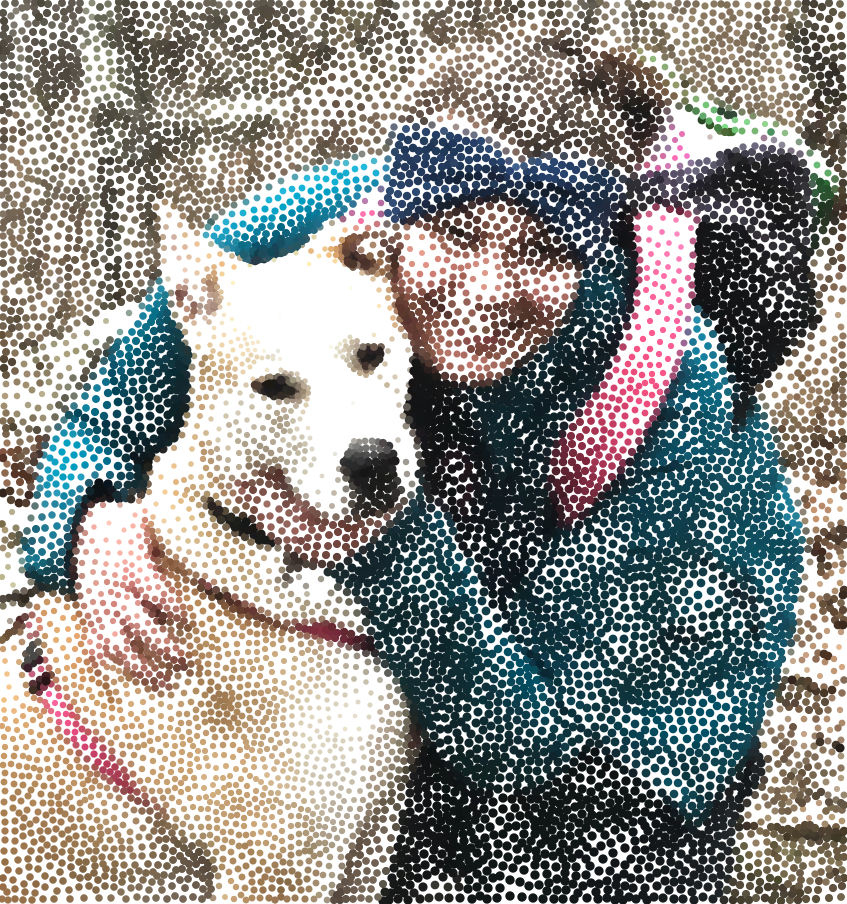
\includegraphics[width=\linewidth]{Emilee-And-Lola-IntensityScaled2-10000}
		\caption{Intensity scaled, 10000 Disks}
		\label{fig:rff2}
	\end{subfigure}
	\begin{subfigure}[b]{.48\linewidth}
		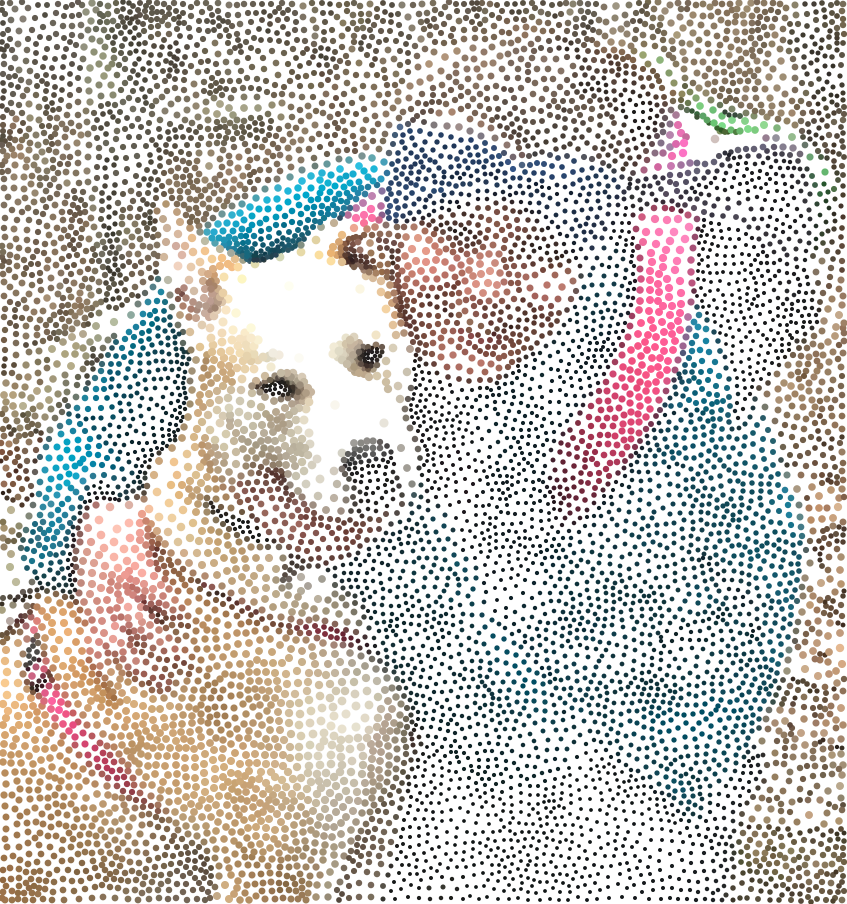
\includegraphics[width=\linewidth]{Emilee-And-Lola-IntensityScaled-10000}
		\caption{Reverse Intensity scaled, 10000 Disks}
		\label{fig:rff3}
	\end{subfigure}
	\caption{Intensity Scaling Example with Girl and Dog}
	\label{fig:rff4}
\end{figure}

We can also apply a regularization process to artificially introduce some variation into the stippling. For example, in the area scaling example, most of the cells are about the same size with a few outliers. In the regularization process, we push the distribution of disk sizes to be more uniform, based on a regularization factor from 0 to 1. The images below show an image of train with negative area scaling and regularization values of 0, 0.3 and 0.8. This effect is enabled by using the \verb|-regularize factor| command. 

\begin{figure}[H]
	\centering
	\begin{subfigure}[b]{.48\linewidth}
		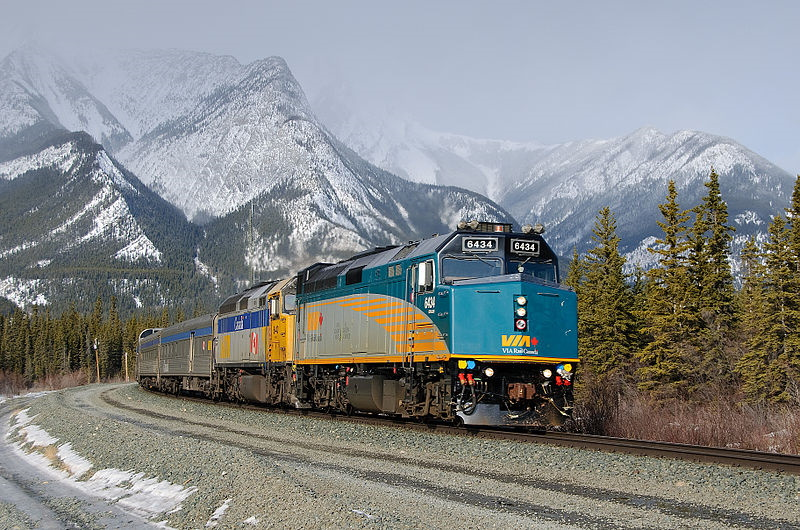
\includegraphics[width=\linewidth]{Train-Canada}
		\caption{Original Image, Train}
		\label{fig:train}
	\end{subfigure}
	\begin{subfigure}[b]{.48\linewidth}
		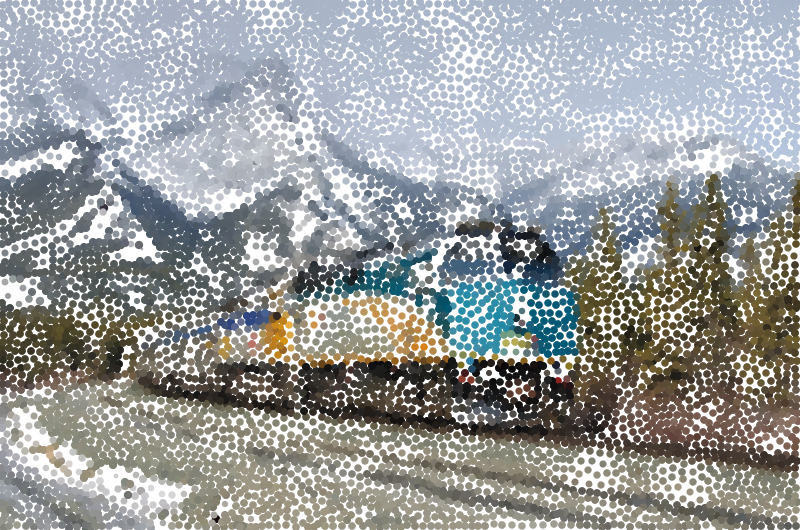
\includegraphics[width=\linewidth]{Train-Canada-8000-1}
		\caption{Reverse area scaling, R = 0}
		\label{fig:train1}
	\end{subfigure}
	\begin{subfigure}[b]{.48\linewidth}
		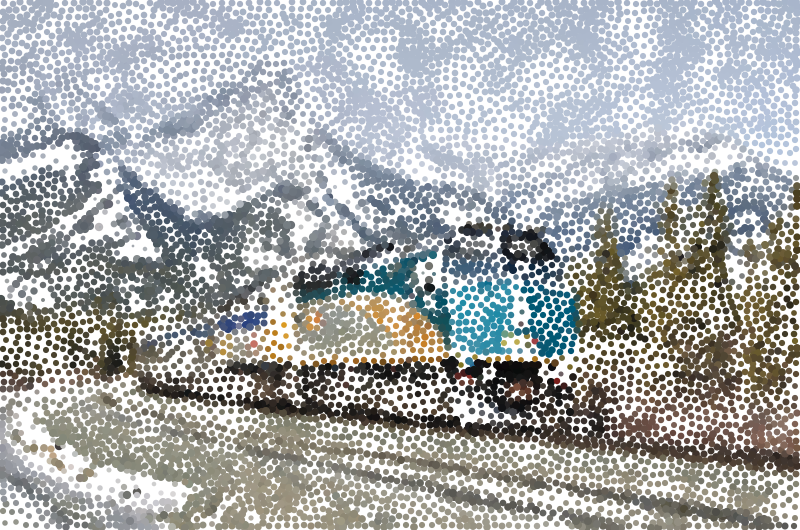
\includegraphics[width=\linewidth]{Train-Canada-8000-2}
		\caption{Reverse area scaling, R = 0.3}
		\label{fig:train2}
	\end{subfigure}
		\begin{subfigure}[b]{.48\linewidth}
		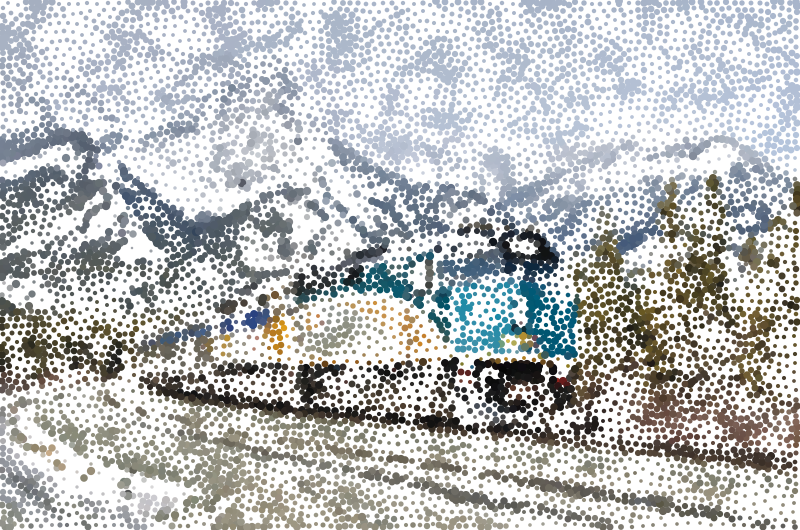
\includegraphics[width=\linewidth]{Train-Canada-8000-3}
		\caption{Reverse area scaling, R = 0.8}
		\label{fig:train3}
	\end{subfigure}
	\caption{Regularization Example with Train}
	\label{fig:mountRusddhmoreEx}
\end{figure}

\subsection{More Dynamic Initial Sampling}

We have also  implemented a tweak to allow greater control over the sampling process. This is enabled with the \verb|-samplingWeight weight| command option. The effect of this is that we are more selective when keeping or throwing away points during the initial sampling. A larger value means that lighter pixels are less likely to get chosen and darker pixels are more likely to be included. In the example below, we see the results for a sampling weight of 0 (uniform distribution), and a sampling weight of 3. Note that we have implemented this as a linear cutoff and large values may lead to an infinite loop because not enough points are eligible for inclusion, so care must be taken.

\begin{figure}[H]
	\centering
	\begin{subfigure}[b]{.52\linewidth}
		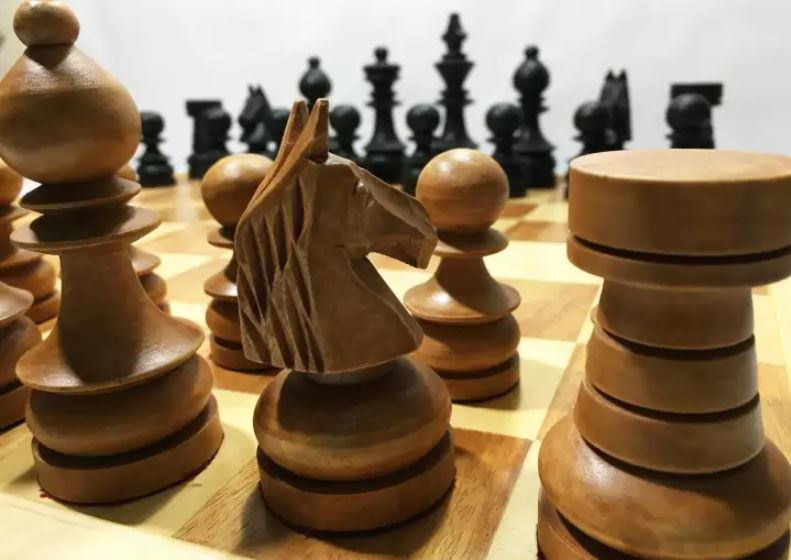
\includegraphics[width=\linewidth]{Chessboard}
		\caption{Original Image, Chessboard}
		\label{fig:gfff}
	\end{subfigure}
	\begin{subfigure}[b]{.48\linewidth}
		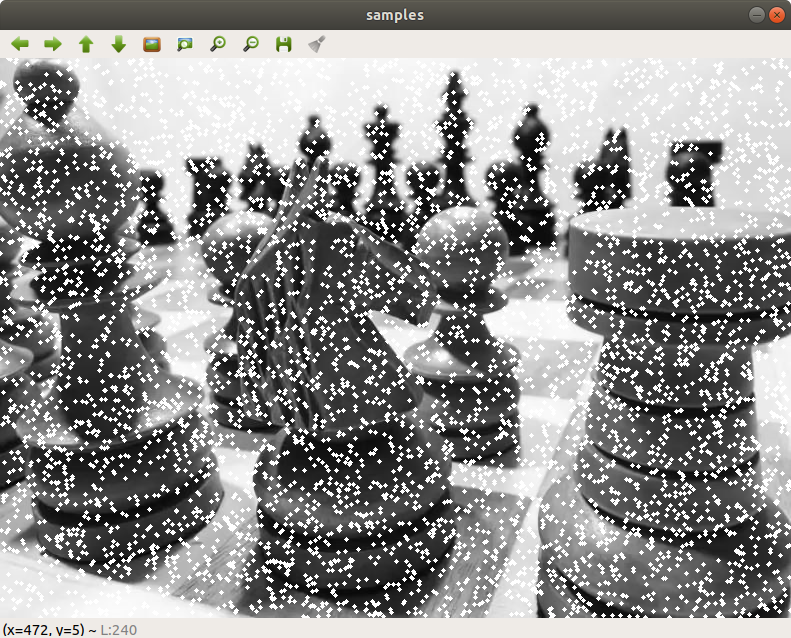
\includegraphics[width=\linewidth]{Chessboard-Points-1}
		\caption{Uniform sample points, 6000 Disks}
		\label{fig:rfff2}
	\end{subfigure}
	\begin{subfigure}[b]{.48\linewidth}
		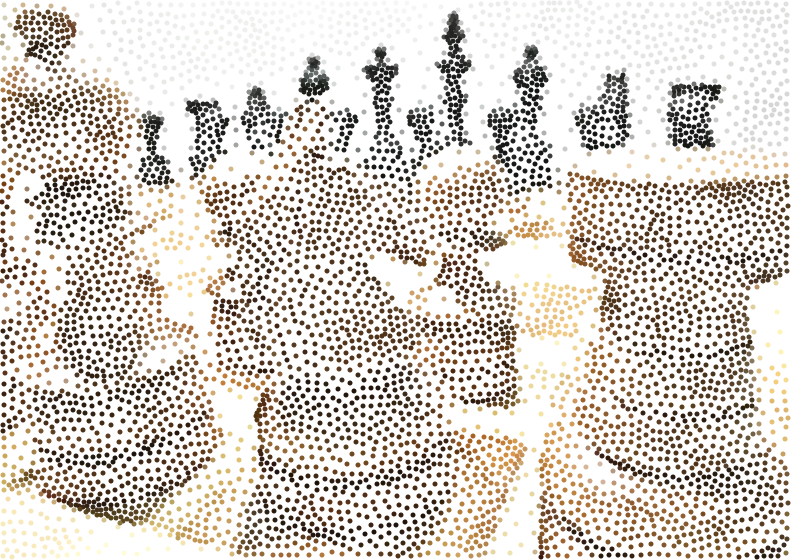
\includegraphics[width=\linewidth]{Chessboard-6000-1}
		\caption{Stippled Chessboard 1, 600 Disks}
		\label{fig:rfff3}
	\end{subfigure}
	\begin{subfigure}[b]{.48\linewidth}
		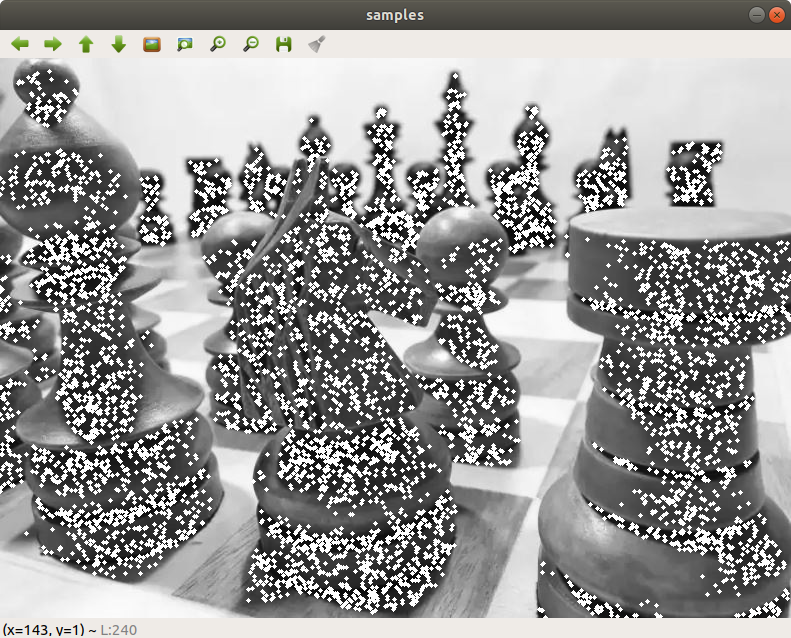
\includegraphics[width=\linewidth]{Chessboard-Points-2}
		\caption{Weighted sample points, 6000 Disks}
		\label{fig:rffdf2}
	\end{subfigure}
	\begin{subfigure}[b]{.48\linewidth}
		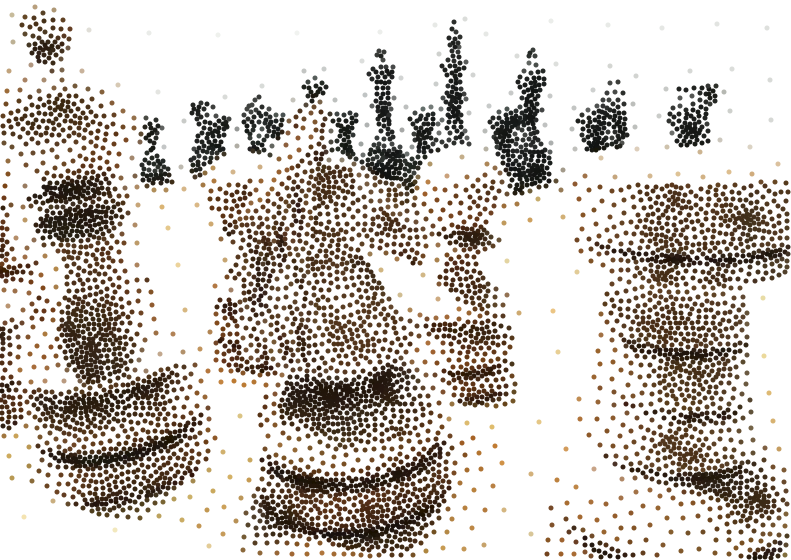
\includegraphics[width=\linewidth]{Chessboard-6000-2}
		\caption{Stippled Chessboard 2, 600 Disks}
		\label{fig:rfffd3}
	\end{subfigure}
	\caption{Initial Sampling Example with Chessboard}
	\label{fig:rfff4}
\end{figure}

\subsection{Edge Detection}

The last feature that we have included in the application is the ability to incorporate information about edges in the input image into the stipple pattern. This enabled by using the \verb|-detectEdges alpha| option. If this is specified, we use OpenCV to detect edges in the input image, using the Sobel operator. Then, we create a linear combination of this output with the grayscale input image, to be used when computing the cell centroids at each step. This helps drag cell centers toward edges in the input image, creating a more well-defined output hedcut, as shown below.

\begin{figure}[H]
	\centering
	\begin{subfigure}[b]{.48\linewidth}
		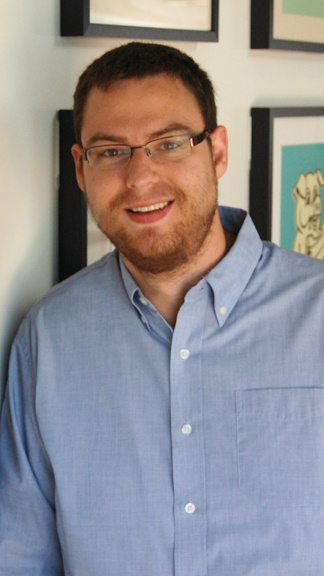
\includegraphics[width=\linewidth]{Portrait}
		\caption{Original Image, Portrait}
		\label{fig:trafin}
	\end{subfigure}
	\begin{subfigure}[b]{.48\linewidth}
		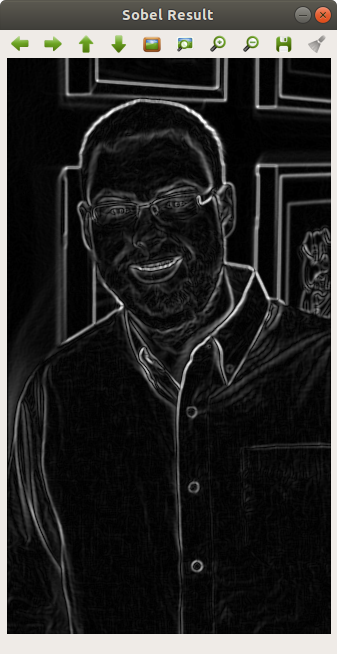
\includegraphics[width=\linewidth]{Portrait-Sobel}
		\caption{Portrait after Sobel Operator (k=3)}
		\label{fig:trxain1}
	\end{subfigure}
	\begin{subfigure}[b]{.48\linewidth}
		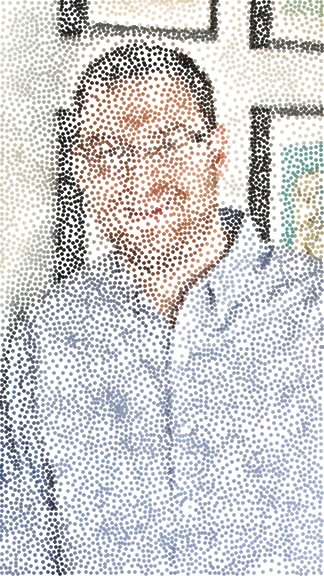
\includegraphics[width=\linewidth]{Portrait-7000-1}
		\caption{Portrait Stippling Default}
		\label{fig:traixn2}
	\end{subfigure}
	\begin{subfigure}[b]{.48\linewidth}
		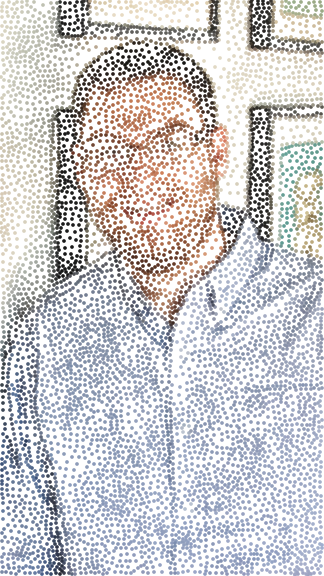
\includegraphics[width=\linewidth]{Portrait-7000-2}
		\caption{Portrait Stippling with Edge Detection}
		\label{fig:traxin3}
	\end{subfigure}
	\caption{Edge Detection Example with Portrait}
	\label{fig:mountRusdxdhmoreEx}
\end{figure}

\section{Conclusion}

This project was a good example of how computer vision and computation geometry algorithms can be applied to interesting real world problems. All of the code that I implemented is completed, and the submitted application runs without any errors. However, there are several things that could be improved or expanded upon. Some examples are:

\begin{itemize}
	\item When using the OpenGL Voronoi diagram option, cells seem to converge somewhat more slowly than using the original method. All of my code is a drop-in replacement for the \verb|vor()| method, so I was a bit confused by this because the \verb|move_sites()| code is exactly the same, regardless of whether the option is on or not.
	\item There are several cases in the code where I have commented out print statements, or dead code. Throughout the course of this project, I spent considerable time experimenting with different ways of doing things and did not have time to clean up everything.
	\item An idea for improvement is to support alpha channels for the disk and background coloring functionality.
	\item Another improvement would be to have support for color scaling, so that stipples could be different shades of the same color (variable intensity). This would look like a grayscale image, but with a different hue.
	\item There are also performance improvements that could be made. For example, I did not implement Fortune's algorithm. In addition, my focus for this project was to enhance the visual aspects of the produced hedcut images, so it is likely that portions of my code could be implemented more cleanly and efficiently.
\end{itemize}

\bibliographystyle{plain}
\bibliography{report}

\end{document}


